% Generated by draw_lafont.py.
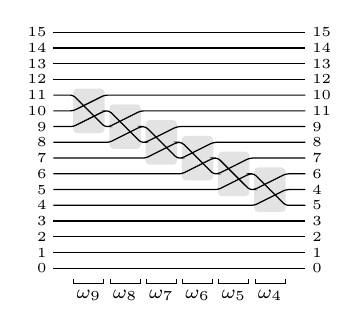
\begin{tikzpicture}[x=1cm,y=1cm,baseline={([yshift=-0.25em]mid)},line width=.45pt]
\coordinate (mid) at (0,-1.500);
\fill[black!11,rounded corners=1.5pt] (0.250,-1.284) rectangle (0.650,-0.716);
\fill[black!11,rounded corners=1.5pt] (0.710,-1.484) rectangle (1.110,-0.916);
\fill[black!11,rounded corners=1.5pt] (1.170,-1.684) rectangle (1.570,-1.116);
\fill[black!11,rounded corners=1.5pt] (1.630,-1.884) rectangle (2.030,-1.316);
\fill[black!11,rounded corners=1.5pt] (2.090,-2.084) rectangle (2.490,-1.516);
\fill[black!11,rounded corners=1.5pt] (2.550,-2.284) rectangle (2.950,-1.716);
\draw[rounded corners=1pt] (0.000,-3.000)--(3.200,-3.000);
\node[anchor=east,font=\tiny,inner sep=0pt] at (-.08,-3.000) {$0$};
\node[anchor=west,font=\tiny,inner sep=0pt] at (3.280,-3.000) {$0$};
\draw[rounded corners=1pt] (0.000,-2.800)--(3.200,-2.800);
\node[anchor=east,font=\tiny,inner sep=0pt] at (-.08,-2.800) {$1$};
\node[anchor=west,font=\tiny,inner sep=0pt] at (3.280,-2.800) {$1$};
\draw[rounded corners=1pt] (0.000,-2.600)--(3.200,-2.600);
\node[anchor=east,font=\tiny,inner sep=0pt] at (-.08,-2.600) {$2$};
\node[anchor=west,font=\tiny,inner sep=0pt] at (3.280,-2.600) {$2$};
\draw[rounded corners=1pt] (0.000,-2.400)--(3.200,-2.400);
\node[anchor=east,font=\tiny,inner sep=0pt] at (-.08,-2.400) {$3$};
\node[anchor=west,font=\tiny,inner sep=0pt] at (3.280,-2.400) {$3$};
\draw[rounded corners=1pt] (0.000,-2.200)--(2.550,-2.200)--(2.950,-2.000)--(3.200,-2.000);
\node[anchor=east,font=\tiny,inner sep=0pt] at (-.08,-2.200) {$4$};
\node[anchor=west,font=\tiny,inner sep=0pt] at (3.280,-2.000) {$4$};
\draw[rounded corners=1pt] (0.000,-2.000)--(2.090,-2.000)--(2.490,-1.800)--(2.550,-1.800)--(2.950,-2.200)--(3.200,-2.200);
\node[anchor=east,font=\tiny,inner sep=0pt] at (-.08,-2.000) {$5$};
\node[anchor=west,font=\tiny,inner sep=0pt] at (3.280,-2.200) {$5$};
\draw[rounded corners=1pt] (0.000,-1.800)--(1.630,-1.800)--(2.030,-1.600)--(2.090,-1.600)--(2.490,-2.000)--(2.550,-2.000)--(2.950,-1.800)--(3.200,-1.800);
\node[anchor=east,font=\tiny,inner sep=0pt] at (-.08,-1.800) {$6$};
\node[anchor=west,font=\tiny,inner sep=0pt] at (3.280,-1.800) {$6$};
\draw[rounded corners=1pt] (0.000,-1.600)--(1.170,-1.600)--(1.570,-1.400)--(1.630,-1.400)--(2.030,-1.800)--(2.090,-1.800)--(2.490,-1.600)--(3.200,-1.600);
\node[anchor=east,font=\tiny,inner sep=0pt] at (-.08,-1.600) {$7$};
\node[anchor=west,font=\tiny,inner sep=0pt] at (3.280,-1.600) {$7$};
\draw[rounded corners=1pt] (0.000,-1.400)--(0.710,-1.400)--(1.110,-1.200)--(1.170,-1.200)--(1.570,-1.600)--(1.630,-1.600)--(2.030,-1.400)--(3.200,-1.400);
\node[anchor=east,font=\tiny,inner sep=0pt] at (-.08,-1.400) {$8$};
\node[anchor=west,font=\tiny,inner sep=0pt] at (3.280,-1.400) {$8$};
\draw[rounded corners=1pt] (0.000,-1.200)--(0.250,-1.200)--(0.650,-1.000)--(0.710,-1.000)--(1.110,-1.400)--(1.170,-1.400)--(1.570,-1.200)--(3.200,-1.200);
\node[anchor=east,font=\tiny,inner sep=0pt] at (-.08,-1.200) {$9$};
\node[anchor=west,font=\tiny,inner sep=0pt] at (3.280,-1.200) {$9$};
\draw[rounded corners=1pt] (0.000,-1.000)--(0.250,-1.000)--(0.650,-0.800)--(3.200,-0.800);
\node[anchor=east,font=\tiny,inner sep=0pt] at (-.08,-1.000) {$10$};
\node[anchor=west,font=\tiny,inner sep=0pt] at (3.280,-0.800) {$10$};
\draw[rounded corners=1pt] (0.000,-0.800)--(0.250,-0.800)--(0.650,-1.200)--(0.710,-1.200)--(1.110,-1.000)--(3.200,-1.000);
\node[anchor=east,font=\tiny,inner sep=0pt] at (-.08,-0.800) {$11$};
\node[anchor=west,font=\tiny,inner sep=0pt] at (3.280,-1.000) {$11$};
\draw[rounded corners=1pt] (0.000,-0.600)--(3.200,-0.600);
\node[anchor=east,font=\tiny,inner sep=0pt] at (-.08,-0.600) {$12$};
\node[anchor=west,font=\tiny,inner sep=0pt] at (3.280,-0.600) {$12$};
\draw[rounded corners=1pt] (0.000,-0.400)--(3.200,-0.400);
\node[anchor=east,font=\tiny,inner sep=0pt] at (-.08,-0.400) {$13$};
\node[anchor=west,font=\tiny,inner sep=0pt] at (3.280,-0.400) {$13$};
\draw[rounded corners=1pt] (0.000,-0.200)--(3.200,-0.200);
\node[anchor=east,font=\tiny,inner sep=0pt] at (-.08,-0.200) {$14$};
\node[anchor=west,font=\tiny,inner sep=0pt] at (3.280,-0.200) {$14$};
\draw[rounded corners=1pt] (0.000,0.000)--(3.200,0.000);
\node[anchor=east,font=\tiny,inner sep=0pt] at (-.08,0.000) {$15$};
\node[anchor=west,font=\tiny,inner sep=0pt] at (3.280,0.000) {$15$};
\draw[line width=.3pt] (0.260,-3.134)--(0.260,-3.194)--(0.640,-3.194)--(0.640,-3.134);
\node[anchor=north,font=\scriptsize,inner sep=2pt] at (0.450,-3.194) {$\omega_{9}$};
\draw[line width=.3pt] (0.720,-3.134)--(0.720,-3.194)--(1.100,-3.194)--(1.100,-3.134);
\node[anchor=north,font=\scriptsize,inner sep=2pt] at (0.910,-3.194) {$\omega_{8}$};
\draw[line width=.3pt] (1.180,-3.134)--(1.180,-3.194)--(1.560,-3.194)--(1.560,-3.134);
\node[anchor=north,font=\scriptsize,inner sep=2pt] at (1.370,-3.194) {$\omega_{7}$};
\draw[line width=.3pt] (1.640,-3.134)--(1.640,-3.194)--(2.020,-3.194)--(2.020,-3.134);
\node[anchor=north,font=\scriptsize,inner sep=2pt] at (1.830,-3.194) {$\omega_{6}$};
\draw[line width=.3pt] (2.100,-3.134)--(2.100,-3.194)--(2.480,-3.194)--(2.480,-3.134);
\node[anchor=north,font=\scriptsize,inner sep=2pt] at (2.290,-3.194) {$\omega_{5}$};
\draw[line width=.3pt] (2.560,-3.134)--(2.560,-3.194)--(2.940,-3.194)--(2.940,-3.134);
\node[anchor=north,font=\scriptsize,inner sep=2pt] at (2.750,-3.194) {$\omega_{4}$};
\end{tikzpicture}
